\chapter{IR using Relational Databases}
\label{ir-using-relational-databases}
\epigraph{``Is this new question a worthy one to investigate?'' This latter question we investigate without further ado, thereby cutting short an infinite regress.}{Alan Turing - 1950}

\begin{Abstract}
\begin{changemargin}{1cm}{1cm}
	In this chapter we first look at the history of using relations databases for information retrieval. We see that their have been many attempts to express information retrieval problems using relational databases. We will highlight one of the latter attempts that revived the idea of expressing bag-of-words ranking functions using SQL. A prototype systems that makes use of these expressions is presented. We show that this system can be used for rapid IR prototyping, and is especially helpful in the context of reproducible information retrieval research.
	We implement many different BM25 variants that have been proposed in the literature, and we do not find the expected effectiveness gains we would expect based on the results presented in the work that proposed them.  
\end{changemargin}
\end{Abstract}


\section{Introduction}
Where commonly information retrieval researchers use inverted indexes as data structures, there is also history of researchers using relational databases for representing the data in information retrieval systems. Different approaches have been tried with varying successes, this chapter will try to summarize what approaches haven been tried in the past decades. Following one of the more recent approaches, studies of ours will be discussed that tried to verify that using relational databases for information retrieval is a valid approach. In particular the advantages for reproducible science will be highlighted. The chapter will be concluded by discussing the pros and cons of these approaches. 

\subsection{Boolean retrieval}
Perhaps the earliest work on using relational databases for information retrieval is the work by Schek and Pistor~\cite{SchekPistor}. In this work the authors recognize that the relational data model is widely accepted as an interface to query structured data, however in cases of unstructured data, like text, it is inconvenient to use. They proposed an extension for the relational model by allowing Non First Normal Form ($NF^2$) relations. This allows for text queries to be more easily expressed, however the systems that can be build in this language are basically boolean retrieval systems. Which at the time worked well, but scoring was not a feature implemented.  
In as similar fashion, Macleod~\cite{macleod} compared the relational model with the inverted index model. He showed how queries of the IBM STAIRS system could be expressed using the relational model. These were however still boolean queries, so scoring using uncertainty was not considered. 

\subsection{Probabilistic Relational Algebra}
Fuhr~\cite{fuhr1996probabilistic} recognized that where databases contain formatted data, IR systems deal with unformatted data and that for this kind of data uncertain inference is required. He proposes to express this uncertainty using a probabilistic relational algebra~\cite{fuhr-pra} (PRA). 
PRA can be considered an extension of the standard relational algebra. 
The basic idea behind PRA is that tuples are being assigned weights, the weight represents the probability that the tuple belongs to the relation. These probabilities gives two advantages. Uncertain information can be expressed and tuples that represent answers to queries can be ordered by the weights that represent the uncertainty. The most certain tuples are ranked to the top. Although these extensions give advantages over boolean retrieval, how to assign these probabilities to for example a document-term pair remains a question.

\subsection{IR on top of a database cluster}
% T. Grabs, K. Bhoem, and H.-J. Schek. PowerDB-IR: scalable information retrieval and storage with a cluster of databases. Knowledge and Information Systems, 6(4):465–505, 2004.
Grabs et al.~\cite{PowerDB-IR} propose PowerDB-IR, which was developed to run IR applications on a scalable infrastructure. Also, it should be able to update the data timely, while also being able to retrieve up-to-date results. The author achieve this by first assigning every document to a category, e.g. sports or news, in their experiments 16 artificial categories are used. For every category a dedicated node is created, which contains tables containing document, inverted list, and statistics tables. 
The system supports both single category, and multi category searches. For single query searchers the following ranking score value is calculated:
\begin{equation}
	\text{RSV}(d,q) = \sum_{t\in q} tf(t, d) \cdot idf(t)^2 \cdot tf(t, q)
\end{equation}
Here $tf(t, d)$ is the term frequency of term $t$ in document $d$, $idf(t)$ is the inverted document frequency of term $t$ (which is squared in this formula), and $tf(t, q)$ is the term frequency of term $t$ in the query text. Calculating this is straightforward, as all statistics necessary is stored on a node. However, when one wants to search on multiple (or all) categories.
The cost of this approach is excessively high, but perhaps it was the first real IR in SQL approach. 

\subsection{Integrating DB + IR}
% S. Chaudhuri, R. Ramakrishnan, and G. Weikum. Integrating DB and IR technologies: What is the sound of one hand clapping? CIDR, 2005.
Chaudhuri et al.~\cite{Chaudhuri2005IntegratingDA} also identify the need for systems that integrate both database and IR functionalities. In their view, database systems are not flexible enough for scoring and ranking, while IR systems can not handle structured data and metadata properly. The authors put together a list of seven requirements that a DB + IR systems should be able to support, of which they identify the following three requirements as the most important:
\begin{enumerate}
	\item \emph{Flexible scoring and ranking.}
	It should be possible to customize the ranking function for different applications; news search might need different ranking functions and settings compared to a web search engine. 
	\item \emph{Optimizability.}
	Queries in a DB+IR systems should, following standard database approaches, have a query optimizer that takes into account the workload and the data characteristics. For example, in the case when only one relevant result is sufficient, the systems should be able to abort when a relevant document is found. 
	\item \emph{Metadata and ontologies.}
	Other than metadata that describes data sources, other metadata that is used for understanding information demands might be needed, this could be for example an ontologie or a lexicon that is used for more effective ranking strategies.
\end{enumerate}
In order to build a system that can support these requirements, the authors identify four alternatives for designing a DB+IR system:
\begin{enumerate}
	\item \emph{On-top-of-SQL.} The IR functionalities are build on top of a SQL engine. The disadvantage of this approach is that it's not easy to customize efficient access for both IR and DB functionalities. 
	\item \emph{Middleware.} In this approach both a SQL engine and an IR engine are ran simultaneously. The two disadvantages of using this approach is that the API needs to talk to two systems, which can have very different design philosophies and the data is not shared between systems, incurring a large overhead and making it harder to combine both functionalities. 
	\item \emph{IR-via-ADT's.} The third approach is building an IR system using abstract data types, the authors argue that this approach makes the system more customizable than the previous approaches. However, the authors also note that optimization in the case of UDF's is very difficult. Also, when programmers need to work with such a system, it has the full complexity of SQL plus the complexity of working with ADT's, and making them efficient. 
	\item \emph{RISC.} The final approach is what the authors prefer; IR functionalities build on top a relational \textit{storage} engine, as described in an earlier work by them~\cite{risc}. The DB+IR systems should then be build on top of this engine. 
\end{enumerate} 
Although the approaches described in this work are interesting, they do not provide prototypes to compare the approaches.

\subsection{Handwritten plans and Array Databases}
% S. H´eman, M. Zukowski, A. de Vries, and P. A. Boncz. MonetDB/X100 at the 2006 TREC terabyte track. TREC, 2006.
H\'eman et al.~\cite{handwritten} participated in the TREC TeraByte track using the relational engine MonetDB/X100. They were able to express ranking functions efficiently and effectively in this system. In their run they used BM25 as a scoring function. In order to reduce the amount of compute necessary, for every document-term pair, the BM25 score was pre-calculated. 
The disadvantage of this approach was that the query plans were not generated from SQL but that they were handwritten. Making this system not easy to use for IR researchers.

% R. Cornacchia, S. H´eman, M. Zukowski, A. de Vries, and P. Boncz. Flexible and efficient IR using array databases. VLDB, 2008.
The same research group~\cite{array-db} also ran experiments on the TREC TeraByte track using the array database SRAM (Sparse Relational Array Mapping). SRAM was able to automatically translate BM25 queries to run them on a relational engine (in particular X100). However SRAM is quite an exotic query language, not used by many people. 

\subsection{Retrieval models only using SQL}
In a more recent work by M\"{u}hleisen et al.~\cite{OldDog} showed that the common used BM25 ranking function can also be easily expressed using SQL, this is done in a similar way as Grabs et al.~\cite{PowerDB-IR} Their work specifically focused on the retrieval efficiency of several systems. They argue that instead of using a custom build information retrieval system using an inverted index, researchers could just simply store their data representations in a column-oriented relational database, and formulate the ranking functions using SQL. They show that their implementation of BM25 in SQL is on par in efficiency and effectiveness compared to systems that use an inverted index. 

There was however an interesting observation in the paper to highlight: All the systems evaluated in this paper implement BM25, there was however a substantial difference between the effectiveness scores produced by these systems, as shown in table~\ref{olddog_results}. The only two systems that achieved the exact same effectiveness score were the two database systems. These two systems were however developed by the same research group.

\begin{table}[!ht]
	\centering
	\caption{Results presented by M\"{u}hleisen et al.~\cite{OldDog}; \texttt{MAP} and \texttt{P@5} on the ClueWeb12 collection are reported for five different systems that run BM25. As shown in the table, only the two database systems achieve the same effectiveness score.}
	\label{olddog_results}
	\begin{tabular}{c c c}
		\toprule
		System &  \texttt{MAP} & \texttt{P@5} \\
		\midrule
		Indri & 0.246 & 0.304 \\
		MonetDB \& VectorWise & 0.225 & 0.276 \\
		Lucene & 0.216 & 0.265 \\
		Terrier & 0.215 & 0.272 \\
		\bottomrule
	\end{tabular}
\end{table}

These results came out as quite a surprise as the authors took specific care to keep document pre-processing identical for all systems, but the observed difference in \texttt{MAP} of 3\% absolute was the largest deviation in score reported.

\subsection{Reproducibility}
Not only did we observe the differences in effectiveness scores for BM25 in the paper by M\"{u}hleisen et al.~\cite{OldDog}. In the SIGIR 2015 Workshop on Reproducibility, Inexplicability, and Generalizability of Results (RIGOR)~\cite{RIGOR} and the Open-Source IR Replicability Challenge (OSIRRC) workshop~\cite{OSIRRC} similar results are observed. See tables~\ref{rigor_results} and~\ref{osirrc_results} respectively.  

\begin{table}
	\centering
	\caption{Results from the RIGOR workshop~\cite{RIGOR}, \texttt{MAP@1000} on the .GOV2 collection is reported for four different systems that run BM25. As shown in the table, all four implementations report a different effectiveness score.}
	\label{rigor_results}
	\begin{tabular}{c c}
		\toprule
		System &  \texttt{MAP@1000} \\
		\midrule
		ATIRE & 0.2902 \\
		Lucene & 0.3029 \\
		MG4J & 0.2994 \\
		Terrier & 0.2697 \\
		\bottomrule
	\end{tabular}
\end{table}

\begin{table}
	\centering
	\caption{Results from the OSIRRC workshop~\cite{OSIRRC}, \texttt{AP}, \texttt{P@30}, and \texttt{NDCG@20} on the robust04 collection are reported for seven different systems that run BM25. As shown in the table, all implementations report (again) a different effectiveness score.}
	\label{osirrc_results}
	\begin{tabular}{c c c c}
		\toprule
		System & \texttt{AP} & \texttt{P@30} & \texttt{NDCG@20} \\
		\midrule
		Anserini (Lucene) & 0.2531 & 0.3102 & 0.4240 \\
		ATIRE & 0.2184 & 0.3199 & 0.4211 \\
		ielab & 0.1826 & 0.2605 & 0.3477 \\
		Indri & 0.2388 & 0.2995 & 0.4041 \\
		OldDog~\cite{olddog-docker} & 0.2434 & 0.2985 & 0.4002 \\
		Pisa & 0.2534 & 0.3120 & 0.4221 \\
		Terrier & 0.2363 & 0.2977 & 0.4049 \\
		\bottomrule
	\end{tabular}
\end{table}

It is not clear why the results between these systems differ this much, many explanations are possible. Examples include; different preprocessing, different hyperparameter settings, different functions for inverse document frequency ( $idf$ ), or erroneous implementation of the ranking function. Using for example non-optimized hyperparameter settings can lead to large gaps in differences between effectiveness scores. Yang et al.~\cite{weak-baselines} showed that in many cases new ranking methods have been proposed that compared results of a new proposed method to a non fine tuned version of BM25, making the results looking better than they actually are. The choices for hyperparameters are often left out of papers, while BM25 is the baseline compared against.
 
Also, 

\section{Variants of BM25}
We~\cite{Kamphuis2020BM25} examined several BM25 variants which will be introduced, how the variant varies from the original formulation as proposed by Robertson et al.~is marked in red. 

\subsubsection{Robertson et al.~\cite{bm25-robertson}} 
The original formulation of BM25 is constructed from two parts, the first part is derived from the binary independence relevance model~\cite{bm25-beyond}, which results in an approximation of the classical inverse document frequency ($ idf $) for a query term $t$:

\begin{equation} 
	w_i^{\text{IDF}} = \log\left(\frac{N-df_t+0.5}{df_t+0.5}\right)
\end{equation}
where $N$ is the size of the collection, and $df_t$ are the number of documents in the collection that contain query term $t$. 

There is however a negative consequence of using this formula for weighing term importance. Lets say there is a collection with $10,000$ documents, then it is possible to plot the ranking score value for each term as shown in fig.~\ref{idf}. The figure shows that the $ idf $ score becomes negative when $df_t > \frac{N}{2}$. This happens for terms that appear in more than half of all documents, e.g.: ``the'' or ``a''. Many systems do not consider these terms when searching by keeping a list of common words that can be ignored (stop words). However, if these words are considered, having a negative $ idf $ would decrease the relevance score of documents that have the query term in the document. Some variations of BM25 deal with this, which will be discussed in following sections. 
 
\begin{figure}
	\caption{Inverse document frequency as used by Robertson et al.~\cite{bm25-robertson}}
	\label{idf}
	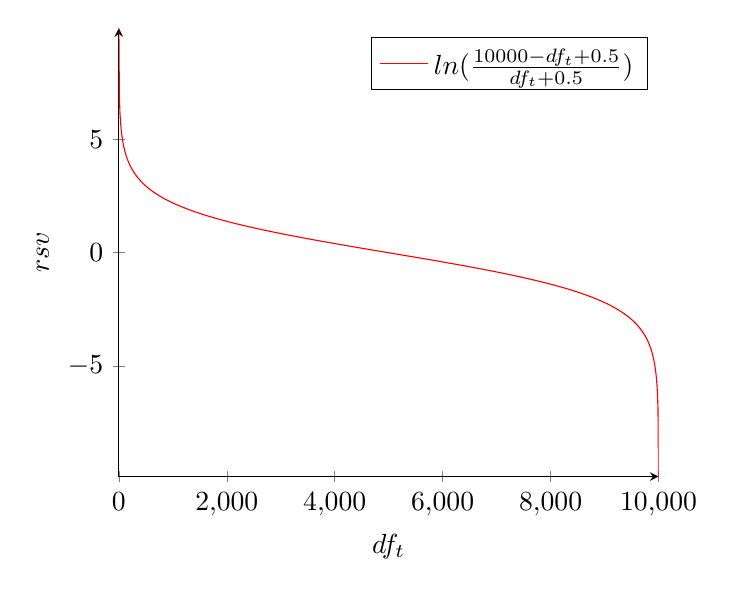
\begin{tikzpicture}
		\begin{axis}[
				axis lines = left,
				xlabel = \(df_t\),
				ylabel = {\(rsv\)},
			]
			%Below the red parabola is defined
			\addplot [
				domain=0:10000, 
				samples=1000, 
				color=red,
			]
			{ln((10000-x+0.5)/(x+0.5))};
			\addlegendentry{\(ln(\frac{10000-df_t+0.5}{df_t+0.5})\)}
		\end{axis}
	\end{tikzpicture}
\end{figure}

The second part of BM25 can be considered as a term frequency weighting $tf$, these two parts are then multiplied to get something like the traditional term frequency - inverse document frequency weighting $tf \times w_i^{\text{IDF}}$.
However the $tf$ in BM25 is extended such that every additional occurrence of a term does not increase the ranking score value as much as the previous one; for example a term being present twice in a document versus once provides more information than a term being present ten times versus nine. For this the following convenient formula as a replacement for \textit{tf} was chosen:

\begin{align}
	\frac{tf}{k+tf} & \text{ where } k>0
\end{align}

This ensures the term frequency does not increase linearly. In the final formulation of BM25 $k$ is written as $k_1$, this is because earlier versions of this ranking formula also had a $k_2$ and $k_3$ parameter. 

Then lastly, a second component is added that can correct for documents being longer than others. It is however not clear how you should deal with documents being longer than others; the author of a document can be verbose, in which case additional term occurrences do not provide anymore information. On the other hand, a long document can be because more relevant information is provided in the document, in which the document is more relevant than its shorter counterpart. For these reasons, the following soft length normalization is introduced:

\begin{align}
	\left(1-b\right) + b \times \left(\frac{L_d}{L_{avg}}\right) & \text{ with } 0 <= b <= 1
\end{align}

When setting $b=1$, full length normalization is used, while if $b=0$ none is used. Combining these parts, including the correction for term frequency and the length normalization we get BM25 as originally proposed by Robertson et al.~\cite{bm25-robertson}:

\begin{equation}
	\label{bm25-robertson}
	\sum_{t\in q} \log\left(\frac{N-df_t+0.5}{df_t+0.5}\right)\cdot\frac{tf_{td}}{k_1\cdot\left(1-b+b\cdot\left(\frac{L_d}{L_{avg}}\right)\right) + tf_{td}}
\end{equation}

\subsubsection{Lucene (default)}
Equation~\ref{lucene-default} shows the variant implemented in Lucene (as of version 8), which introduces two main differences highlighted in red. First, since the $idf$ component of Robertson et al. is negative when:

\begin{equation}
	df_t > \frac{N}{2} 
\end{equation}

To avoid negative values in all possible cases, Lucene adds a constant one before calculating the $log$ value. 

Second, the document length used in the scoring function is compressed (in a lossy manner) to a one byte value, denoted $L_{d\text{lossy}}$. With only 256 distinct document lengths, Lucene can pre-compute the value of

\begin{equation}
	k_1 \cdot \left(1-b+b\cdot\left(\frac{L_{d\text{lossy}}}{L_{avg}}\right)\right)
\end{equation}

for each possible length, resulting in fewer computations at query time.

\begin{equation}
	\label{lucene-default}
	\sum_{t\in q}\log\left(\mathbf{\begingroup\color{ruhuisstijlrood}1 +\endgroup} \frac{N-df_t+0.5}{df_t+0.5}\right)\cdot\frac{tf_{td}}{k_1\cdot\left(1-b+b\cdot\left(\frac{L_{d \mathbf{\begingroup\color{ruhuisstijlrood}lossy\endgroup}}}{L_{avg}}\right)\right)+tf_{td}}
\end{equation}

\subsubsection{Lucene (accurate)}

Equation~\ref{lucene-accurate} represents our attempt to measure the impact of Lucene’s lossy document length encoding. We implemented a variant that uses exact document lengths, but is otherwise identical to the Lucene default.

\begin{equation}
	\label{lucene-accurate}
	\sum_{t\in q}\log\left(\mathbf{\begingroup\color{ruhuisstijlrood}1 +\endgroup} \frac{N-df_t+0.5}{df_t+0.5}\right)\cdot\frac{tf_{td}}{k_1\cdot \left(1-b+b\cdot\left(\frac{L_d}{L_{avg}}\right)\right)+tf_{td}}
\end{equation}

\subsubsection{ATIRE~\cite{ATIRE}}
Equation~\ref{atire-variant} shows BM25 as implemented by ATIRE; it implements the $idf$ component of BM25 as $log(N/df_{t})$, which also avoids negative values. The TF component is multiplied by $k_1+1$ to make it look more like the classic Robertson/Sparck Jones (RSJ) weight~\cite{RSJ}; this has no effect on the resulting ranked list, as all scores are scaled linearly with this factor.

\begin{equation}
	\label{atire-variant}
	\sum_{t\in q}\log\left(\mathbf{\begingroup\color{ruhuisstijlrood}\frac{N}{df_t}\endgroup}\right)\cdot\frac{\mathbf{\begingroup\color{ruhuisstijlrood}\left(k_1 + 1\right)\endgroup}\cdot tf_{td}}{k_1\cdot\left(1-b+b\cdot\left(\frac{L_{d}}{L_{avg}}\right)\right)+tf_{td}}
\end{equation}

\subsubsection{BM25L~\cite{bm25l}}
BM25L, as shown in equation~\ref{bm25l}, builds on the observation that BM25 penalizes longer documents too much compared to shorter ones. The $idf$ component differs, to avoid negative values. The TF component is reformulated as:
\begin{equation}
	\frac{\left(k_1+1\right)\cdot c_{td}}{k_1+c_{td}}  
\end{equation}
with 

\begin{equation}
	c_{td} = \frac{tf_{td}}{1 - b + b \cdot \left(\frac{L_d}{L_{avg}}\right)}  
\end{equation}
The $c_{td}$ component is further modified by adding a constant $\delta$ to it, boosting the score for longer documents. The authors report using $\delta = 0.5$ for highest effectiveness.

\begin{equation}
	\label{bm25l}
	\sum_{t\in q} \log\left(\mathbf{\begingroup\color{ruhuisstijlrood}\frac{N+1}{df_t + 0.5}\endgroup}\right)\cdot\frac{\mathbf{\begingroup\color{ruhuisstijlrood}(k_1 + 1)\endgroup}\cdot(c_{td} \mathbf{\begingroup\color{ruhuisstijlrood}+ \delta\endgroup})}{k_1 + (c_{td} \mathbf{\begingroup\color{ruhuisstijlrood}+ \delta\endgroup})}
\end{equation}

\subsubsection{BM25+~\cite{bm25+}}
BM25+, as shown in equation~\ref{bm25+}, encodes a general approach for dealing with the issue that ranking functions unfairly prefer shorter documents over longer ones. The proposal is to add a lower-bound bonus when a term appears at least one time in a document. The difference with BM25L is a constant $\delta$ to the TF component. The $idf$ component is again changed to a variant that disallows negative values.

\begin{equation}
	\label{bm25+}
	\sum_{t\in q} \log\left(\mathbf{\begingroup\color{ruhuisstijlrood}\frac{N+1}{df_t}\endgroup}\right)\cdot\left(\frac{\mathbf{\begingroup\color{ruhuisstijlrood}\left(k_1 + 1\right)\endgroup}\cdot tf_{td}}{k_1\cdot\left(\left(1-b\right)+b\cdot\left(\frac{L_d}{L_{avg}}\right)\right)+tf_{td}}+\mathbf{\begingroup\color{ruhuisstijlrood}\delta\endgroup}\right)
\end{equation}

\subsubsection{BM25-adpt~\cite{bm25-adpt}}
BM25-adpt is an approach that varies $k_1$ per term (i.e., uses term specific $k_1$ values). In the original formulation of BM25, $k_1$ can be considered a hyperparameter that regulates the increase of score for additional occurrences of a term; $k_1$ ensures that every additional occurrence gets discounted as it provides less information. However, Lv and Zhai argued that this does not necessary have to be the case. If there are much fewer documents that have $t+1$ occurrences versus $t$, it should provide more information compared to when the number of documents are almost equal. In order to find the optimal term-specific $k_1$ value, the authors want to maximize the information gain for that particular query term. 
This is done by first identifying the probability of selecting a document randomly from the collection that contains term $q$ at least once in a document as:

\begin{equation}
	p(1|0,q) = \frac{df_t+0.5}{N+1}
\end{equation}

The probability of a term occurring one more time is defined as:

\begin{equation}
p(t+1|t,q) = \frac{df_{t+1}+0.5}{df_t+1}
\end{equation}

In both these formulas, $1$ and $0.5$ are added for smoothing to avoid zero probabilities. Then the information gain from $t$ to $t+1$ occurrences is computed as, subtracting the initial probability: 

\begin{equation}
	G^t_q = \log_2\left(\frac{df_{t+1} + 0.5}{df_t+1}\right) - \log_2 \left(\frac{df_{t} + 0.5}{N+1}\right)
\end{equation}

Here $df_t$ is not defined as a normal document frequency, but based on the length normalized term frequency:

\begin{equation}
	df_t = 
	\begin{cases}
		|D_{t|c_{td}\geq t-0.5}| & t > 1\\ 
		df(q) & t = 1\\
		N & t = 0
	\end{cases}
\end{equation}

In this case $df(q)$ is the ``normal'' document frequency, and $c_{td}$ is the same as in BM25L (pivoted method for length normalization~\cite{ctd}):

\begin{equation}
	c_{td} = \frac{tf_{td}}{1-b+b\cdot\left(\frac{L_d}{L_{avg}}\right)}
\end{equation}

This means the following: $df_t$ is equal to number of documents in the collection when $t = 0$, it is equal to the ``normal'' document frequency when $t = 1$, and otherwise it will be the number of documents that have at least $t$ occurrences of the term (rounded up) using the pivoted method $c_{td}$. 

Then, the information gain is calculated for $t \in \{0,\cdots,T\}$,until $G^t_q > G^{t+1}_q$. This threshold is chosen as a heuristic: When $t$ becomes large, the estimated information gain can be very noisy. So $T$ is chosen as the smallest value that breaks the worst burstiness rule~\cite{burstiness_rule} (the information gain starts decreasing). The optimal value for $k_1$ is then determined by finding the value for $k_1$ that minimizes the following equation:
\begin{equation}
	k'_1 = \argmin_{k_1} \sum_{t=0}^{T}\left(\frac{G^t_q}{G^1_q} - \frac{(k_1+1)\cdot t}{k_1+t}\right)^2
\end{equation}

Essentially, this gives a value for $k_1$ that maximizes information gain for that specific term; $k_1$ and $G^1_q$ are then plugged into the BM25-adpt formula: 

\begin{equation}
	\label{bm25-adpt}
	\sum_{t\in q}\mathbf{\begingroup\color{ruhuisstijlrood}G_q^1\endgroup}\cdot\frac{\mathbf{\begingroup\color{ruhuisstijlrood}\left(k'_1+1\right)\endgroup}\cdot tf_{td}}{\mathbf{\begingroup\color{ruhuisstijlrood}k'_1\endgroup}\cdot\left(\left(1-b\right)+\cdot\left(\frac{L_d}{L_{avg}}\right)\right)+tf_{td}}
\end{equation}

We found that the optimal value of $k_1$ is actually not defined for about 90\% of the terms. A unique optimal value for $k_1$ only exists when $t > 1$ while calculating $G^t_q$. For many terms, especially those with a low $df$, $G^t_q > G^{t+1}_q$ occurs before $t > 1$. In these cases, picking different values for $k_1$ has virtually no effect on retrieval effectiveness. For undefined values, we set $k_1$ to $0.001$, the same as Trotman et al.~\cite{trotman-bm25}


\subsubsection{TF $l\circ\delta\circ p\times$IDF~\cite{tf-ldp-idf}}
TF$l\circ\delta\circ p\times$IDF, as shown in equation \ref{tf-ldp-idf}, models the non-linear gain of a term occurring multiple times in a document as:
\begin{equation}
	1+\log\left(1+\log\left(tf_{td}\right)\right) 
\end{equation}

To ensure that terms occurring at least once in a document get boosted, the approach adds a fixed component $\delta$, following BM25+. These parts are combined into the TF component using the pivoted method for length normalization~\cite{ctd}:

\begin{equation}
	c_{td} = \frac{tf_{td}}{1-b+b\cdot\left(\frac{L_d}{L_{avg}}\right)}
\end{equation}

The same IDF component as in BM25+ is used, which gives us TF$l\circ\delta\circ p\times$IDF: 

\begin{equation}
	\label{tf-ldp-idf}
	\sum_{t\in q}\log\left(\mathbf{\begingroup\color{ruhuisstijlrood}\frac{N+1}{df_t}\endgroup}\right)\cdot\left(\mathbf{\begingroup\color{ruhuisstijlrood}1+\log\endgroup}\left(\mathbf{\begingroup\color{ruhuisstijlrood}1+\log\endgroup}\left(\mathbf{\begingroup\color{ruhuisstijlrood}c_{td}+\delta\endgroup}\right)\right)\right)
\end{equation}

\section{Experiments}
Our experiments were conducted using Anserini (v0.6.0) on Java 11 to create
an initial index, and subsequently using relational databases for rapid prototyping, which we dub ``OldDog''~\cite{olddog-docker} after M\"{u}hleisen et al.~\cite{OldDog}; following that work use MonetDB as well. Evaluations with Lucene (default) and Lucene (accurate) were performed directly in Anserini; the latter was based on previously-released code that we updated and incorporated into Anserini.\footnote{http://searchivarius.org/blog/accurate-bm25-similarity-lucene} The inverted index was exported from Lucene to OldDog, ensuring that all experiments share exactly the same document processing pipeline (tokenization, stemming, stopword removal, etc.). While exporting the inverted index, we precalculate all $k_1$ values for BM25-adpt as suggested by Lv and Zhai~\cite{bm25-adpt}. As an additional verification step, we implemented both Lucene (default) and Lucene (accurate) in OldDog and compared results to the output from Anserini. We are able to confirm that the results are the same, setting aside unavoidable differences related to floating point precision. All BM25 variants are then implemented in OldDog as minor variations upon the original SQL query provided in M\"{u}hleisen et al.~\cite{OldDog}. The term-specific parameter optimization for the adpt variant was already calculated during the index extraction stage, allowing us to upload the optimal $(t, k)$ pairs and directly use the term-specific $k$ values in the SQL query. The advantage of our experimental methodology is that we did not need to implement a single new ranking function from scratch. % todo All the SQL variants implemented for this paper can be found on GitHub. 

The experiments use three TREC newswire test collections: TREC Disks 4 and 5, excluding Congressional Record, with topics and relevance judgments from the TREC 2004 Robust Track (Robust04); the New York Times Annotated Corpus, with topics and relevance judgments from the TREC 2017 Common Core Track (Core17); the TREC Washington Post Corpus, with topics and relevance judgments from the TREC 2018 Common Core Track (Core18). Following standard experimental practice, we assess ranked list output in terms of average precision (\texttt{AP}) and precision at rank 30 (\texttt{P@30}). The parameters shared by all models are set to $k_1$ = 0.9 and $b$ = 0.4, Anserini’s defaults. The parameter $\delta$ is set to the value reported as best in the corresponding source publication. 

All experiments were run on a Linux desktop (Fedora 30, Kernel 5.2.18, SELinux enabled) with 4 cores (Intel Xeon CPU E3-1226 v3 @ 3.30 GHz) and 16 GB of main memory; the MonetDB 11.33.11 server was compiled from source using the \texttt{---enable-optimize} flag.

% todo Table 2 presents the effectiveness scores for the implemented retrieval functions on all three test collections.
% todo Table 3 presents the average retrieval time per query in milliseconds (without standard deviation for Anserini, which does not report time per query). MonetDB uses all cores for both inter-and intraquery parallelism, while Anserini is single-threaded.

\section{Results}
Table~\ref{bm25_variant_results} shows the effectiveness scores of the different BM25 variants.  

\begin{table}
	\centering
	\caption{Effectiveness scores different BM25 variants, all were implement as SQL queries, so the underlying data representations are exactly the same. }
	\label{bm25_variant_results}
	\begin{tabular}{l c c c c c c}
		\toprule
		&\multicolumn{2}{c}{Robust04}&\multicolumn{2}{c}{Core17}&\multicolumn{2}{c}{Core18}\\
		&\texttt{AP}&\texttt{P@30}&\texttt{AP}&\texttt{P@30}&\texttt{AP}&\texttt{P@30}\\
		\midrule
		{\small Robertson et al.} & .2526 & .3086 & .2094 & .4327 & .2465 & \textbf{.3647} \\ 
		{\small Lucene (default)} & .2531 & .3102 & .2087 & .4293 & .2495 & .3567 \\ 
		{\small Lucene (accurate)} & .2533 & .3104 & .2094 & .4327 & .2495 & .3593 \\ 
		{\small ATIRE} & .2533 & .3104 & .2094 & .4327 & .2495 & .3593 \\ 
		{\small BM25L} & .2542 & .3092 & .1975 & .4253 & \textbf{.2501} & .3607 \\ 
		{\small BM25+} & .2526 & .3071 & .1931 & .4260 & .2447 & .3513 \\ 
		{\small BM25-adpt} & \textbf{.2571} & \textbf{.3135} & \textbf{.2112} & .4133 & .2480 & .3533\\ 
		{\small $\text{TF}_{l\circ\delta\circ p}\times\text{IDF}$} & .2516 & .3084 & .1932 & \textbf{.4340} & .2465 & .3647\\ 
		\bottomrule
	\end{tabular}
\end{table}

The observed differences in effectiveness are very small and can be fully attributed to variations in the scoring function; our methodology fixes all other parts of the indexing pipeline (tag cleanup, tokenization, stopwords, etc.). Both an ANOVA and Tukey’s HSD show no significant differences between any variant, on all test collections. This confirms the findings of Trotman et al.~\cite{trotman-bm25}: effectiveness differences are unlikely an effect of the choice of the BM25 variant. Across the IR literature, we find that differences due to more mundane settings (such as the choice of stopwords) are often larger than the differences we observe here. Although we find no significant improvements over the original Robertson et al.~\cite{bm25-robertson} formulation, it might still be worthwhile to use a variant of BM25 that avoids negative ranking scores.

You might have caught that the effectiveness scores of both ATIRE and Lucene (accurate) are exactly the same. This is not a mistake. As explained, the $k_1+1$ in ATIRE scales the scores linearly and does not effect the ranking. So the only difference that can change the effectiveness scores are the different $idf$ functions, but these are practically the same, especially when a collection has a large number of documents ($N$):

\begin{align}
	\log\left(\frac{N}{df_t}\right) &= \log\left(\frac{N-df_t+df_t}{df_t}\right) \\
									&= \log\left(\frac{N-df_t}{df_t} + \frac{df_t}{df_t}\right) \\
									&= \log\left(\frac{N-df_t}{df_t} + 1\right) \\
									&\approx \log\left(\frac{N-df_t+0.5}{df_t+0.5} + 1\right)
\end{align}

Table~\ref{bm25_effiency} presents the average retrieval time per query in milliseconds (without standard deviation for Anserini, which does not report time per query). MonetDB uses all cores for both inter- and intra-query parallelism, while Anserini is single-threaded.

\begin{table}
	\centering
	\caption{Average retrieval time per query in ms: Anserini (top) and OldDog (bottom)}
	\label{bm25_effiency}
	\begin{tabular}{l | c c c}
		\toprule
		&Robust04&Core17&Core18\\
		\midrule
		Lucene (default)&52&111&120\\
		Lucene (accurate)&55&115&123\\
		\midrule
		Robertsen et al.&$158\pm25$&$703\pm162$&$331\pm96$\\
		Lucene (default)&$157\pm24$&$699\pm154$&$326\pm90$\\
		Lucene (accurate)&$157\pm24$&$701\pm156$&$324\pm88$\\
		ATIRE&$157\pm24$&$698\pm159$&$331\pm94$\\
		BM25L&$158\pm25$&$697\pm160$&$333\pm96$\\
		BM25+&$158\pm25$&$700\pm160$&$334\pm96$\\
		BM25-adpt&$158\pm24$&$700\pm157$&$330\pm92$\\
		TF$_{l\circ\delta\circ p}\times$IDF&$158\pm24$&$698\pm158$&$331\pm96$ \\
		\bottomrule
	\end{tabular}
\end{table}

Comparing Lucene (default) and Lucene (accurate), we find negligible differences in effectiveness. However, the differences in retrieval time are also negligible, which calls into question the motivation behind the original length approximation. Currently, the similarity function and thus the document length encoding are defined at index time. Storing exact document lengths would allow for different ranking functions to be swapped at query time more easily, as no information would be discarded at index time. Accurate document lengths might additionally benefit downstream modules that depend on Lucene. We therefore suggest that Lucene might benefit from storing exact document lengths.
 
\section{Do BM25 variants matter?}
In summary, the previous sections describe a double reproducibility study: it methodologically validates the usefulness of databases for IR prototyping claimed by M\"{u}hleisen et al.~\cite{OldDog} and performed a large-scale study of BM25 to confirm the findings of Trotman et al.~\cite{trotman-bm25}. Returning to our original motivating question regarding the multitude of BM25 variants: ``Does it matter?'', we can conclude that the answer appears to be ``no, it does not''.